	\paragraph{Présentation}
		La loi de distribution de Zipf est une loi empirique (basée sur l'observation) qui veut que le mot le plus fréquent est, à peu de chose près, 2 fois plus fréquent que le $2^{eme}$, 3 fois plus fréquent que le $3^{eme}$ etc.\\

		La formulation finale de la $1^{ere}$ loi de Zipf est la suivante :

		\begin{align*}
				|mot| = constante \times rang(mot)^{k \approx 1}
		\end{align*}

		avec \emph{$|mot|$} la fréquence d'apparition d'un mot, \emph{constante} une valeur propre à chaque texte, \emph{rang(mot)} la place du mot dans le tri décroissant par fréquence d'apparition et \emph{k} un coefficient proche de 1. 

	\paragraph{Développement}
		Afin de pouvoir utiliser les résultats de cette distribution dans ce projet, j'ai développé un ensemble de fonctions sur un corpus "\emph{reconnu}". Mon choix s'est porté sur le corpus \emph{Brown} (voir \ref{Brown_corpus}) présent dans la librairie \emph{nltk}. Ce corpus contient environ 500 documents contenant 1 millions de mot en anglais.\\

		Le processus d'analyse se fait sur 2 versions de ce corpus.
		\begin{itemize}
			\item la première version contient tous les mots sans modifications
			\item le seconde version contient tous les mots sans les \emph{stopwords}
		\end{itemize}
		Les \emph{stopwords} sont des mots qui n'ont pas ou peu de signification dans un texte. Ces mots sont retirés dans la $2^e$ version pour voir l'effet d'une réduction sur la distribution de Zipf. \\

		Les paragraphes ci-dessous détaillent les étapes du développement :

		\subparagraph{Étape 1 - Ordonner les mots}
			La première étape est de compter les occurrences de tous les mots des 2 corpus et de les ranger en fonction de leur nombre d’occurrence. 
			\begin{lstlisting}[title=Triage des mots]
def frequence_mot(bag, freq=None):
    """
    Calcule la frequence de chaque mot dans un sac de mot
    :param bag: <list> - liste de tous les mots d'un texte
    :param freq: <dict> - dictionnaire avec {<str> mot: <int> frequence}
    :return: <dict> - dictionnaire avec la frequence par mot {mot: frequence}
    """
    if freq is None:
        freq = {}
    for mot in bag:
        freq[mot] = freq.get(mot, 0) + 1
    return freq

def classement_zipf(dico):
    """
    Trie un dictionnaire de mots : occurence et leur assigne un rang en fonction du nombre d'occurence
    :param dico: <dict> dictionnaire de mot: occurrences
    :return: <list> {"rang": <int>, "mot": <str>, "frequence": <int>}
    """
    ranked = []
    for rang, couple in enumerate(sorted(dico.items(), key=lambda item: item[1], reverse=True), start=1):
        ranked.append({"rang": rang,
                       "mot": couple[0],
                       "frequence": couple[1]})

    return ranked \end{lstlisting}


    		On obtient les représentations suivantes: 
		\begin{figure}[H]
				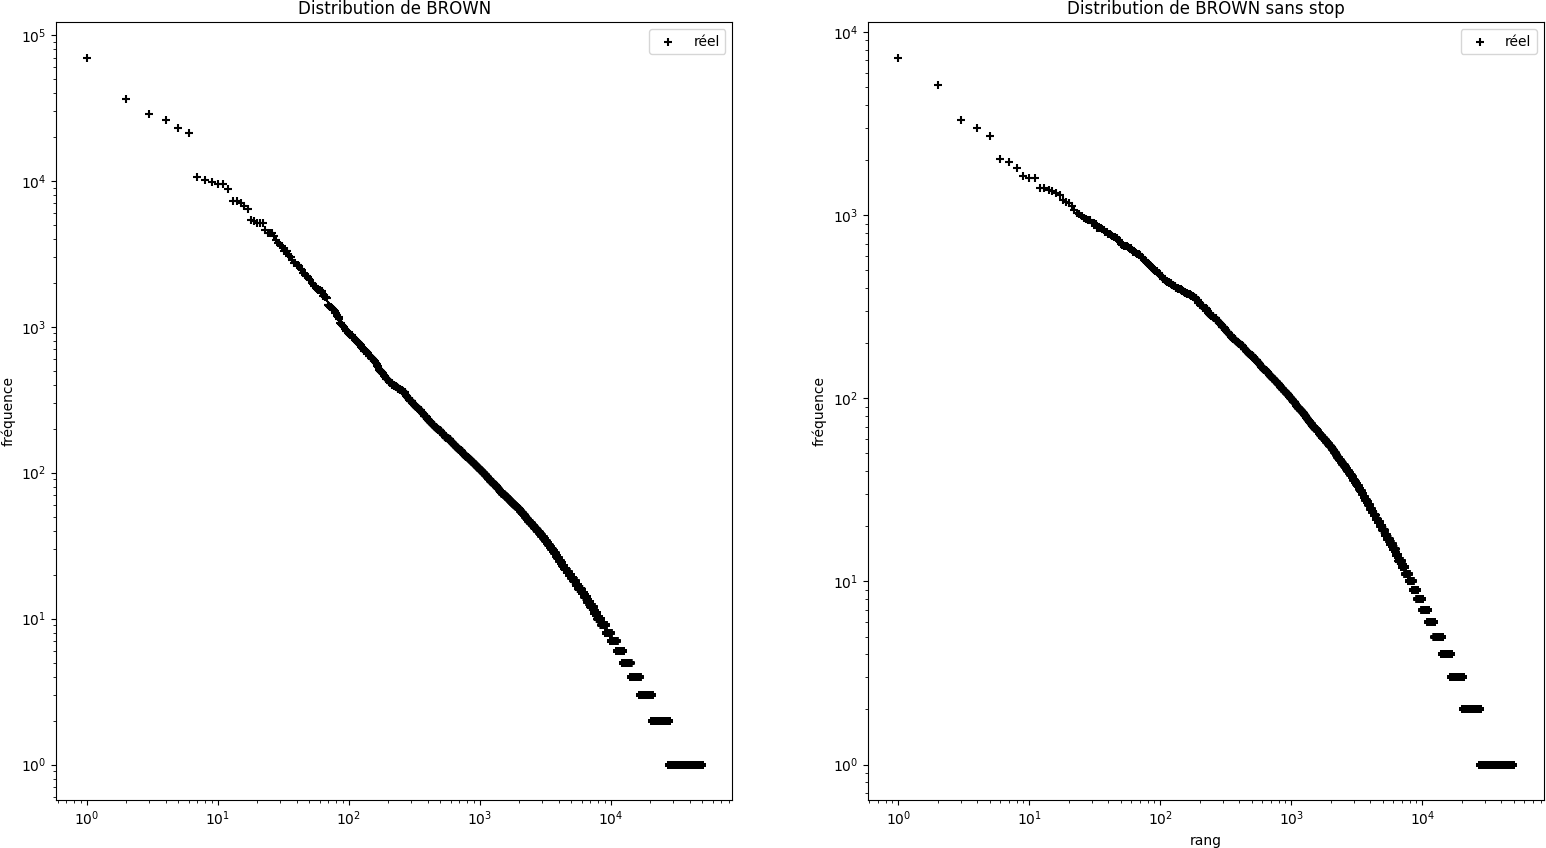
\includegraphics[width=\linewidth]{img/distribZipf.png}
				\caption{Distribution de Zipf pour les deux corpus}
		\end{figure}    		

    		\begin{itemize}
    			\item Nombre de mots dans brown:	mots: 49398	occurences: 1012528
    			\item Nombre de mots dans brown stop:	mots: 49383	occurences: 578837\\
    		\end{itemize}

    		La distribution de la version complète du corpus semble à première vue plus fidèle à la représentation classique de la distribution de Zipf. 

		\subparagraph{Etape 2 - calcul de la constante}
			Le premier paramètre qu'il faut déterminer est la \emph{constante}. Pour ce faire j'effectue le calcul suivant pour tous les mots :

			\begin{align*}
				constante = |mot| \times rang(mot)
			\end{align*}

			On obtient une liste de toutes les constantes théoriques pour chaque mot selon son rang.
			De cette liste, nous allons extraire la moyenne et la médiane.

			\begin{figure}[H]
				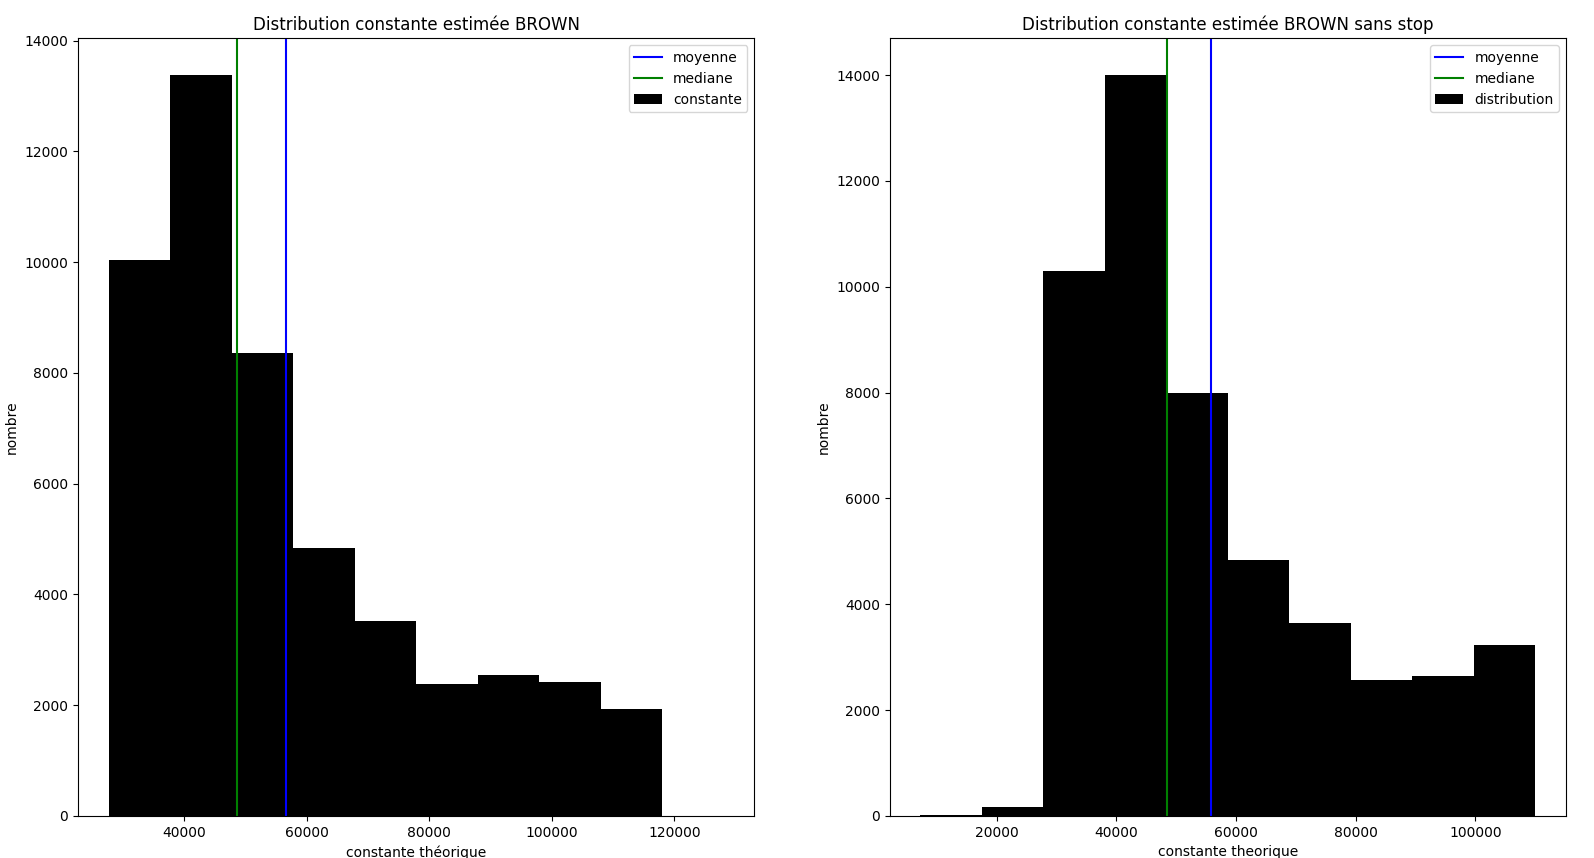
\includegraphics[width=\linewidth]{img/distribContTh.png}
				\caption{Distribution des constantes théoriques pour les deux corpus}
			\end{figure}

			On voit qu'il y a une majorité de mots donnant une constante brute comprise entre $20.000$ et $60.000$. Dans les deux corpus
			La différence entre les moyennes et médianes des deux corpus n'est pas flagrante :
			\begin{itemize}
				\item Brown moyenne: 56525.81, médiane: 48601.50
				\item Brown (- stopwords) moyenne: 55809.97, médiane: 48494.00
			\end{itemize}


		\subparagraph{Etape 3 - recherche du coefficient}
			Le coefficient $k$ permet d'ajuster le résultat, et pourra éventuellement donner une indication de complexité. La recherche de $k$ se fera sur les deux corpus avec utilisant les moyennes et médianes.\\

			Pour ce faire nous allons:

			\begin{enumerate}
				\item Faire la liste de tous les coefficients possibles dans l'intervalle $[0.86, 1.3]$ avec un pas de $0.01$\footnote{les bornes et le pas sont totalement arbitraire afin d'obtenir un graphique présentable}.
				\item Calculer toutes la fréquences théoriques de tous les rangs avec tous les coefficients possibles en utilisant les constantes moyenne et médiane de chaque corpus.
				\item Calculer la moyenne des coûts absolus entre les fréquences théoriques par coefficient avec la fréquence réelle observée pour chaque corpus.\\
			\end{enumerate}

			Le couple coefficient/constante avec le coup minimal sera retenu pour l'utilisation dans la phase de \emph{feature engineering}. \\	

			\begin{lstlisting}[title=Fonctions utilisées dans la recherche du coefficient]
def zipf_freq_theorique(constante, rang, coef):
    """
    Calcul la frequence theorique d'un mot selon son rang, la constante du texte et un coeficiant d'ajustement
    :param constante: <int> constante determinee par la distribution de Zipf
    :param rang: <int> rang du mot selon sa frequence
    :param coef: <float> variable d'ajustement
    :return: <float> frequence theorique zipfienne
    """
    return constante / (rang ** coef)

def cout(l1, l2, methode):
    """
    Calcul le cout de l'ecart entre les elements de l1 et le l2, place par place
    :param l1: <list> liste d'entier
    :param l2: <liste> liste d'entier
    :param methode: <str> methode de calcul du cout
    :return: <float> cout selon methode
    """
    if len(l1) != len(l2):
        print("Erreur, fonction cout: l1 & l2 de taille differente", file=sys.stderr)
        return None

    if len(l1) == 0:
        print("Erreur, fonction cout: liste vide", file=sys.stderr)

    if methode.lower() not in ['absolue', 'carre', 'racine']:
        print("Erreur, fonction cout - methode '{}' inconnue".format(methode), file=sys.stderr)
        return None

    if methode.lower() == 'absolue':
        return np.mean([abs(x-y) for x, y in zip(l1, l2)])

    if methode.lower() == 'carre':
        return np.mean([(x-y)**2 for x, y in zip(l1, l2)])

    if methode.lower() == 'racine':
        return np.sqrt(np.mean([(x-y)**2 for x, y in zip(l1, l2)]))

    return None\end{lstlisting}

			\begin{lstlisting}[title=Calcul des fréquences par coefficient]
    ls_coef = list(np.arange(0.86, 1.3, 0.01))
    zbmo_th = {coef: [stats.zipf_freq_theorique(zb_const_moyen, r, coef) for r in zb_rang] for coef in ls_coef}
    zbme_th = {coef: [stats.zipf_freq_theorique(zb_const_median, r, coef) for r in zb_rang] for coef in ls_coef}
    zbmoth_cmoy = [stats.cout(zb_freq, zbmo_th[coef], 'absolue') for coef in ls_coef]
    zbmeth_cmoy = [stats.cout(zb_freq, zbme_th[coef], 'absolue') for coef in ls_coef]

    zbsmo_th = {coef: [stats.zipf_freq_theorique(zbs_const_moyen, r, coef) for r in zbs_rang] for coef in ls_coef}
    zbsme_th = {coef: [stats.zipf_freq_theorique(zbs_const_median, r, coef) for r in zbs_rang] for coef in ls_coef}
    zbsmoth_cmoy = [stats.cout(zbs_freq, zbsmo_th[coef], 'absolue') for coef in ls_coef]
    zbsmeth_cmoy = [stats.cout(zbs_freq, zbsme_th[coef], 'absolue') for coef in ls_coef] \end{lstlisting}

		La recherche du coefficient nous retourne les éléments suivants:
			\begin{figure}[H]
				\includegraphics[width=\linewidth]{img/coutZipf.png}
				\caption{Coût absolu moyen par coefficient}
			\end{figure}

			\begin{itemize}
				\item Coût min brown moyenne: 5.93, median: 7.01
				\item Coût min brown (- stopwords) moyenne: 6.95, median: 6.46
				\item Coefficient min brown moyenne: 0.92, median: 0.91
				\item Coefficient min brown (- stopwords) moyenne: 0.97, median: 0.95
			\end{itemize}

	\paragraph{Résultats}

		Le tableaux ci dessous rappelle les données récupérées au long de la recherche:
		\begin{center}
			\begin{tabular}{|l|c|c|}
				\hline
				& BROWN avec stopwords & BROWN sans stopwords \\
				\hline
				nombre de mots uniques & 49398 & 49383 \\
				\hline
				nombre de mots total & 1012528 & 578837 \\
				\hline
				Constante moyenne & 56525.81 & 55809.97 \\
				\hline
				Constante médiane & 48601.50 & 48494.00 \\
				\hline
				Coefficient avec moyenne & 0.92 & 0.97 \\
				\hline
				Cout du coefficient moyenne & 5.93 & 6.95 \\
				\hline
				Coefficient avec médiane & 0.91 & 0.95 \\
				\hline
				Cout du coefficient médiane & 7.01  & 6.46 \\
				\hline
			\end{tabular}		
		\end{center}

		D'après les données il est possible de dire que l'on obtient de meilleurs résultats si on conserve tous les mots du corpus. Dans ce cas l'utilisation de la moyenne des constantes génère un taux d'erreur plus faible que la médiane.\\

		Ci-dessous la représentation des fréquences théoriques avec le coefficient optimal pour chaque corpus et chaque méthode. On voit que la courbe de la constante moyenne sur le corpus brute est celle qui suit le mieux les données réelles.
		\begin{figure}[H]
			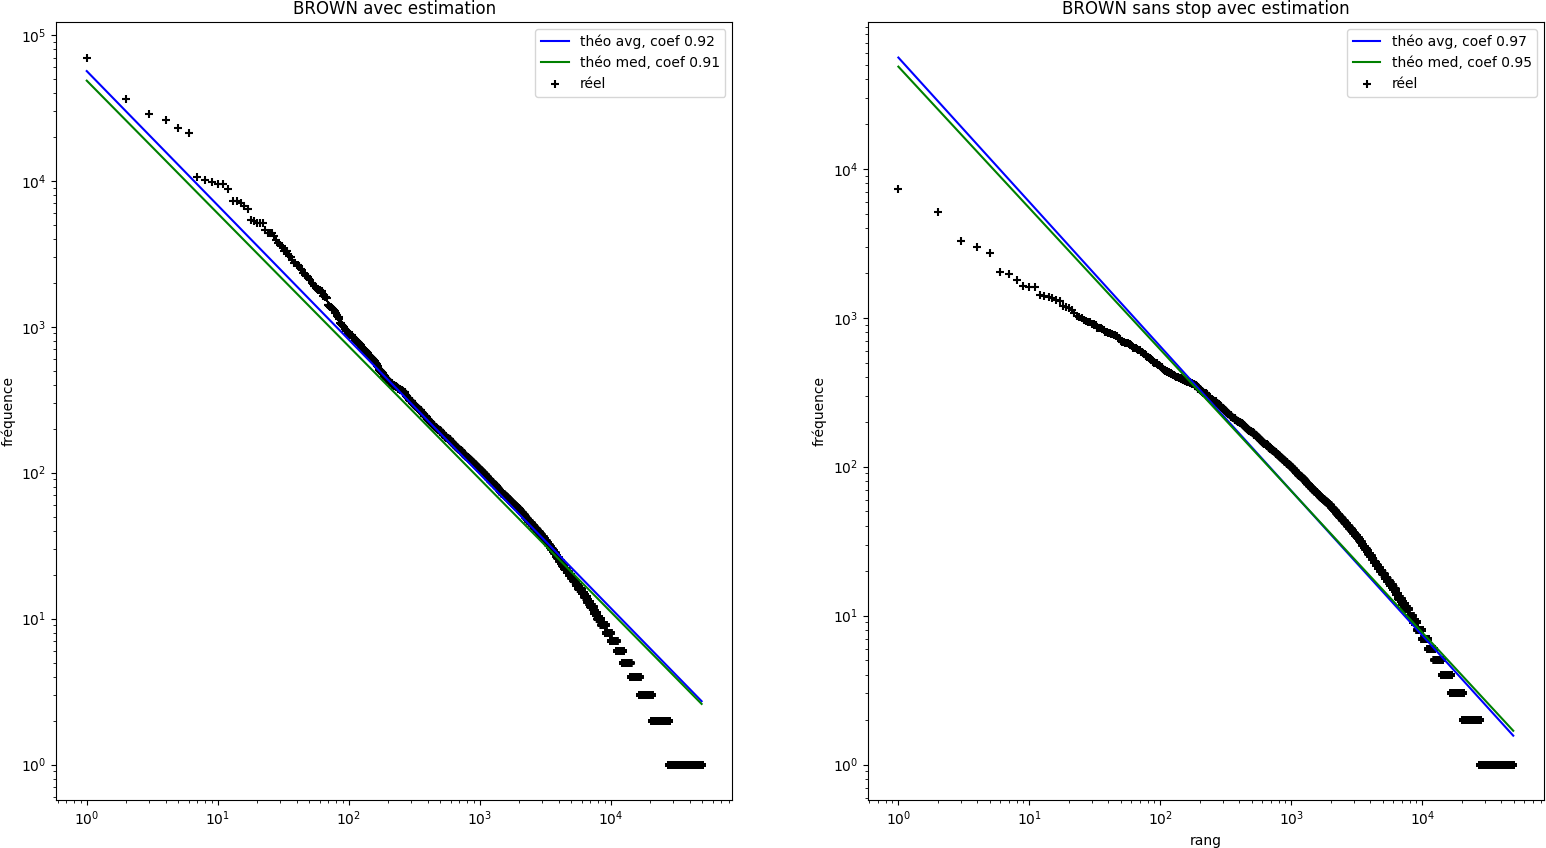
\includegraphics[width=\linewidth]{img/zipfFin.png}
			\caption{Distribution de Zipf avec les estimations}
		\end{figure}

		En conclusion, j'utiliserais la moyenne des constantes sur un document complet afin de déterminer le coefficient dans ma recherche de spam.